\documentclass{article}
\usepackage[utf8]{inputenc}


\title{Search Algorithms}
\author{(Sam) TsunSing Leung }
\date{3/18/2016}

\usepackage{natbib}
\usepackage{graphicx}
\usepackage{subfig}
\usepackage[margin=0.7in]{geometry}

\begin{document}

\maketitle{Final Results}

\section{\large Results' Accuracy}

    In the final results, Hill climbing with random restarts did the best, while simulated annealing came in second, and normal hill climbing came in last. This is most likely due to the shape being like a valley with not many small bumps in it. With hill climbing, it would get very close to the global minima in most cases, but would not be accurate and consistent due to it sometimes running into small bumps. However, hill climbing with random restarts gets rid of this issue by doing multiple iterations of hill climbing which would give it a higher chance of not going a path that was not blocked by a rare bump. Simulated annealing on the other hand, was in the middle of the two because it stayed consistent due to its nature, but was unable to reach the global minima due to the heavy amount of resources needed to lower the step-size. However, it was very consistent with its answers which was also very close to the global minima.

\section{\large Search Speed}

    Hill Climb took the shortest time to run. Depending on the number of restarts for hill climbing with restarts and the max temperature and step-size for simulated annealing, one took longer than the other depending on these factors. A higher number of restarts causes hill climbing with random restarts to take longer due to the higher amount of times it has to run, while the lower step-size and higher temperature of simulated annealing caused it to take longer to run as the search would have to go through more iterations before the temperature went to zero.

\section{\large Future Changes}

    If i were to make any changes to better this program, I would have used dictionaries to store the x and y coordinates of the different states instead of placing each of them into its own variable. I also would have merged the main parts of the 3 programs due to its similar nature, with an extra parameter to take in the type of search to do so the program can end up with less lines overall.

\section{\large Plots of Search Algorithms}

\begin{figure}[h!]
  \centering
  \subfloat[Single Hill Climb]{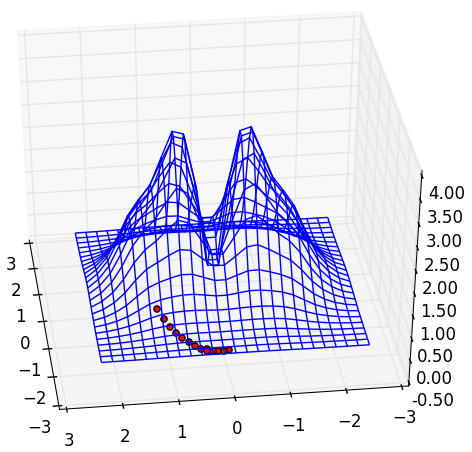
\includegraphics[width=0.3\textwidth]{hill_climb.png}\label{fig:f1}}
  \hfill
  \subfloat[Hill Climbing with Random Restarts]{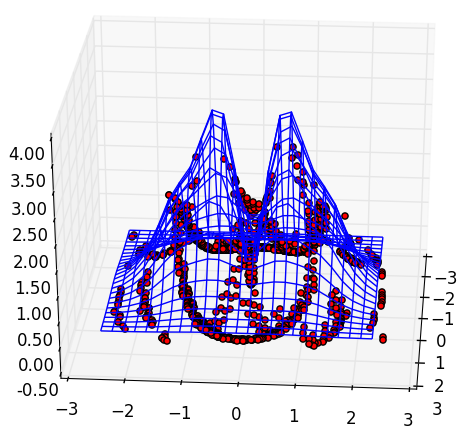
\includegraphics[width=0.3\textwidth]{hill_climb_w_restart.png}\label{fig:f2}}
  \hfill
  \subfloat[Simulated Annealing]{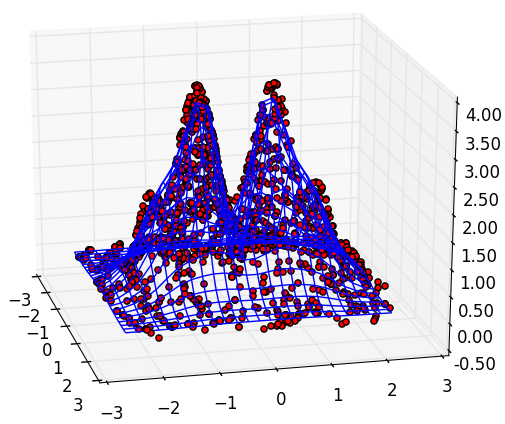
\includegraphics[width=0.3\textwidth]{simulated_annealing.png}\label{fig:f2}}
\end{figure}


\end{document}
